\documentclass[10pt]{article}

\usepackage[margin=0.82in]{geometry}
\usepackage{amsmath,amssymb,booktabs,graphicx,microtype,placeins}
\usepackage[hidelinks]{hyperref}
\usepackage{xcolor}

\newcommand{\E}{\mathbb{E}}
\newcommand{\R}{\mathbb{R}}
\newcommand{\KL}{\mathrm{KL}}

\title{Single-Sequence-Native Disentanglement of\\Marginal Entropy and Sparse Categorical Interactions}
\author{Working draft}
\date{July 2026}

\begin{document}
\maketitle

\begin{center}
\fbox{\parbox{0.92\linewidth}{\textbf{Empirical-log status.}
This long draft is retained as a research record.  An independent review found a target-builder
alias and a teacher/student gauge mismatch that make downstream architecture conclusions
provisional.  The current authoritative manuscript is \texttt{theory\_main.tex}; experiments
are paused while the common-gauge mathematics and prior-art boundary are refined.}}
\end{center}

\begin{abstract}
Protein Transformers encode strong structural signals, but commonly used pair scores mix
single-site conservation, sequence motifs, directional information flow, and genuine
non-additive interactions.  We study an architecture that treats this separation as a
training-time structural constraint rather than a post-hoc correction.  The model accepts a
single sequence by default.  An optional multiple-sequence alignment (MSA) is used only as a
teacher for site marginals and relation scores.  A marginal branch predicts a site-specific
amino-acid distribution and its entropy.  A narrow continuous indexer ranks position pairs,
top-$k$ creates computational sparsity, and a pair-conditioned branch produces signed
categorical fields only for selected pairs.  The fields are projected into a weighted zero-sum
gauge defined by the marginal distribution, making the one-body and pairwise function spaces
non-overlapping.  On a 3CNBA pilot with a frozen ESM-2 8M backbone, a
rank-32 interaction head reconstructs a finite-mutation categorical response map with a
Spearman correlation of 0.895 and attains long-range contact precision $P@L=0.792$, compared
with $0.800$ for the teacher, while only 7.0\% of pair gates exceed 0.5.  On a separate
383-family benchmark, hard binary residual targets are inferior to continuous
entropy-normalized ranking.  A pair-MLP indexer reaches held-out long-range $P@L=0.063$,
compared with contact prevalence 0.026.  Removing four sequence-level phylogeny modes
improves the MSA teacher contact average precision, but neither global nor pair-conditioned
factor heads faithfully reconstruct full categorical covariance across families.  We therefore
define the final layer directly through additive marginal logits and sparse interaction fields,
and treat MSA block reconstruction as optional auxiliary supervision rather than the execution
contract of the architecture.  In a two-seed end-to-end masked-token demo, dense-to-sparse
training makes top-$k$ conversion stable, but the sparse model remains statistically tied with a
local background and below a Transformer; the typed interaction contribution is not
reproducible across seeds.  A marginal-orthogonal task-gradient objective does produce a
replicated improvement over a frozen background, but an equally constrained site-only residual
matches the pair model.  We therefore introduce an explicitly non-additive double-mutation
teacher.  After separating family-level interaction scale from the weighted-zero-sum field
shape, a two-sided projected pair model explains 6.16\% and 4.17\% of held-out-family shape
variance in two seeds, while a site-only control explains none.  The paired projected-pair
improvement has 95\% family-bootstrap interval $[0.0168,0.0875]$.  This establishes a weak but
identifiable pair signal.  Static strength prediction fails, but a gate conditioned on the current
masked-task hidden state reaches held-out Spearman 0.725/0.700 and top-10\% average precision
0.651/0.644.  Dynamic value states do not improve categorical shape, motivating separate
task-conditioned routing keys and stable marginal-orthogonal values.
Joint adaptation of a contiguous-segment router recovers 92.5\% of dense neighbors at an
estimated 62.3\% of dense vector work and improves teacher KL in both seeds, but true-residue
cross-entropy remains seed-dependent.  A full conditional-response scan further shows that
nonlocal interaction energy is sparse but not contiguous in primary-sequence coordinates,
rejecting sequence blocks as the default protein interaction partition.  This motivates a
content-balanced interaction-tile router rather than an axial or sequence-block sparse layer.
The implemented 32-candidate router recovers 96.7\% of dense neighbors at 28.5\% estimated
vector work on validation.  Across three model seeds and 2,052 targets from 57 untouched test
families, the original-value router retains 97.0\% recall and reproducibly improves teacher KL.
Its true-residue cross-entropy gain is positive in all three seeds but has 95\% interval
$[-0.00159,0.00755]$.  Freezing or jointly adapting the categorical value does not significantly
improve this result.  Thus candidate routing is no longer the main empirical bottleneck;
generalization of the categorical message remains unresolved, and stable values with dynamic
routing are the supported default.  A gauge-preserving nonlinear set aggregator further improves
teacher fidelity in all three seeds but reduces the mean true-residue gain relative to simple
addition, indicating that aggregation capacity alone does not repair the supervision mismatch.
The teacher beats the local background on only 54.2\% of test targets; filtering distillation to
teacher-better training examples reduces teacher matching but still does not improve test CE.
A two-teacher consensus is a significantly better masked-residue predictor, yet rebuilding the
full conditional-response basis from consensus targets changes interaction CE by only
$0.000126$ with an interval crossing zero.  A leave-query-out MSA log-odds teacher, in contrast,
has a strong calibrated test CE gain, but the present site-shared value basis cannot learn its
categorical fields across families.
\end{abstract}

\section{Introduction}

Statistical protein models often reduce a categorical coupling block $J_{ij}(a,b)$ to a
non-negative scalar score such as a Frobenius norm.  Such scores can be dominated by a
Perron mode associated with site entropy or conservation, obscuring the sparse residue pairs
that carry structural information \cite{wang2024disentanglement}.  In a symmetric
non-negative matrix, average product correction can approximately remove this leading mode.
Transformer statistics are more difficult: attention is directional and row stochastic,
hidden-state and logit responses are signed, and the relevant interaction signal can occupy
multiple categorical modes rather than one leading eigenvector.

Our initial experiments suggest a decomposition
\begin{equation}
T(x) = B_{\mathrm{marginal}}(x) + I_{\mathrm{interaction}}(x),
\end{equation}
where the first term is large and predictable from motif/PSSM information, while the second
term is smaller but contact-rich.  This motivates an architecture that provides distinct
computational primitives for these terms.

Recent efficiency work makes it important to state what is not new.  Multi-head Latent
Attention (MLA) compresses per-token keys and values but retains softmax token-to-token
attention \cite{deepseekv2,deepseekv3}.  DeepSeek Sparse Attention (DSA) uses a lightweight
indexer to select a small subset of historical tokens for exact attention
\cite{deepseekv32}.  DeepSeekMoE separates shared and routed computation
\cite{deepseekmoe}, and Engram separates static lookup memory from dynamic computation
\cite{engram}.  Native Sparse Attention (NSA) combines compressed blocks, selected fine-detail
blocks, and a local window in a natively trainable hardware-aligned operator \cite{nsa}.
Our proposed contribution is not low-rank KV compression, top-$k$ routing,
or shared experts.  It is an explicit, identifiable separation between a marginal categorical
function and a signed typed pair interaction.

\section{Problem formulation}

Let $x=(x_1,\ldots,x_L)$ be a single protein sequence and let $q=20$ be the amino-acid
alphabet size.  A marginal branch predicts
\begin{equation}
p_i(a\mid x)=\operatorname{softmax}_a b_i(a),
\qquad
H_i=-\sum_a p_i(a\mid x)\log p_i(a\mid x).
\end{equation}
When an MSA is available during training, its empirical PSSM supervises $p_i$.  Without an
MSA, $p_i$ is an amortized single-sequence estimate learned across protein families.

The interaction branch predicts blocks $G_{ij}\in\R^{q\times q}$.  For each site define
\begin{equation}
P_i = I - \mathbf{1}p_i^\top.
\end{equation}
Given an unconstrained block $S_{ij}$, its marginal-free component is
\begin{equation}
G_{ij}=P_iS_{ij}P_j^\top.
\label{eq:weighted-gauge}
\end{equation}
It follows directly that
\begin{equation}
p_i^\top G_{ij}=0,
\qquad
G_{ij}p_j=0.
\label{eq:orthogonality}
\end{equation}
For uniform $p_i$, Eq.~\ref{eq:weighted-gauge} reduces to the conventional zero-sum convention
for Potts parameters.  Here ``gauge'' refers only to additive parameter non-identifiability, not
to spin-reversal symmetry or to a lattice gauge field; below we call the projected result
reference-centered.
For non-uniform $p_i$, it is a functional ANOVA projection under the site-specific reference
distribution.

Equation~\ref{eq:orthogonality}, rather than zero empirical correlation between interaction
strength and entropy, is our definition of disentanglement.  Structural interactions can be
stronger at conserved sites, so forcing the scalar interaction norm to be uncorrelated with
$H_i$ can remove genuine signal.

\section{Architecture}

\subsection{Single-sequence backbone and marginal branch}

The prototype uses frozen single-sequence ESM-2 residue states $h_i\in\R^d$.  A full model
would replace or augment selected Transformer layers, but the factor-head experiment isolates
the proposed representation from backbone training effects.  The marginal branch is
\begin{equation}
b_i=W_b\operatorname{LN}(h_i),
\qquad p_i=\operatorname{softmax}(b_i).
\end{equation}

\subsection{Normalized categorical factors}

For rank $R$, the model predicts raw factors $U_i(a,r)$.  We apply weighted centering
\begin{equation}
\widetilde U_i(a,r)
=U_i(a,r)-\sum_c p_i(c)U_i(c,r),
\end{equation}
followed by a per-site, per-mode RMS normalization.  This prevents site-specific factor norms
from becoming a hidden entropy channel.

The more general primitive does not require a pair representation.  For any residual logits
$z_i(a)$, define
\begin{equation}
R_i(a)=z_i(a)-\sum_c p_i(c)z_i(c),\qquad p_i^\top R_i=0.
\label{eq:site-residual}
\end{equation}
This site-level marginal-orthogonal residual is a strict control for all pairwise constructions.
Experiments below show that it explains the observed task-gradient benefit; sparse pair fields
must outperform Eq.~\ref{eq:site-residual} before they can be claimed as necessary.

\subsection{Continuous relation index and \texorpdfstring{top-$k$}{top-k} routing}

A narrow symmetric indexer predicts a continuous score
\begin{equation}
s_{ij}=f_{\mathrm{idx}}(h_i,h_j)=s_{ji},\qquad
\mathcal N_i=\operatorname{TopK}_{j}\,s_{ij}.
\label{eq:indexer}
\end{equation}
The score is not interpreted as a calibrated edge probability.  Binary three-MAD targets
discard useful ordering information, while a fixed nonzero probability creates a dense Perron
mode.  Sparsity is instead an explicit compute budget: the narrow indexer may score all pairs,
but the expensive typed operator is evaluated only for $j\in\mathcal N_i$.  This follows the
engineering pattern of DSA; the distinct component is the entropy-normalized teacher and the
typed value operator below.

\subsection{Pair-conditioned typed interaction}

A symmetric pair network predicts a non-negative amplitude $\alpha_{ij}$ and a signed mode
direction $\widehat\kappa_{ij,r}$ with unit RMS.  The interaction is
\begin{equation}
G_{ij}(a,b)
=\alpha_{ij}\sum_{r=1}^{R}\widehat\kappa_{ij,r}
\widetilde U_i(a,r)\widetilde U_j(b,r).
\label{eq:factorization}
\end{equation}
This construction guarantees block-transpose symmetry
$G_{ij}(a,b)=G_{ji}(b,a)$ and Eq.~\ref{eq:orthogonality}.  Pair-specific $\widehat\kappa$
is necessary because one site can participate in chemically different interactions with
different partners; a single global mode scale is too restrictive across protein families.
The epistasis experiment below further indicates that amplitude and categorical geometry
should be trained as separate objects.  We write
\begin{equation}
G_{ij}=\alpha_{ij}\widehat G_{ij},\qquad
p_i^\top\widehat G_{ij}=0,\quad \widehat G_{ij}p_j=0,
\label{eq:amplitude-shape}
\end{equation}
where $\widehat G_{ij}$ is normalized during shape supervision and $\alpha_{ij}$ is predicted by
a distinct strength gate.  Otherwise large cross-family variation in interaction scale dominates
the loss and obscures the more transferable signed field geometry.

For an observed sequence, the layer produces additive categorical logits
\begin{equation}
\ell_i(a)=b_i(a)+\sum_{j\in\mathcal N_i}G_{ij}(a,x_j).
\label{eq:additive-logits}
\end{equation}
If $x_j$ is masked, it is replaced by its marginal distribution $p_j$.  The expected message is
then exactly zero because $G_{ij}p_j=0$.  Thus unknown context cannot leak marginal information
through the interaction path.  The interaction logits may also be projected back to hidden
width and added beside a cheap local/background convolution, yielding a stackable replacement
for selected Transformer layers.

\subsection{Optional MSA teacher}

The model input remains a single sequence.  If an MSA is available during training, it defines
a marginal teacher and a relation-ranking teacher:
\begin{align}
p_i^{\mathrm{MSA}}(a) &= \frac{1}{N}\sum_n \mathbf{1}[x_i^{(n)}=a],\\
T_{ij}^{\mathrm{int}} &=
\mathcal{P}_{p^{\mathrm{MSA}}}
\left(
T_{ij}^{\mathrm{real}}-
\E_{\widetilde X\sim Q_{\mathrm{null}}}T_{ij}^{\widetilde X}
\right),
\end{align}
where $\mathcal{P}_p$ denotes weighted categorical projection and block-transpose
symmetrization.  At inference, the MSA can be absent; the predicted $p_i$ defines the gauge.
An optional MSA adapter may add a family-specific residual, but is not required for execution.

For empirical MSA covariance, finite depth, phylogeny, and marginal diversity make nearly
every pair nonzero.  Define
\begin{align}
d_i &= 1-\|p_i^{\mathrm{MSA}}\|_2^2,\qquad
m_{ij}=\|T_{ij}^{\mathrm{int}}\|_F/q,\\
r_{ij} &= m_{ij}/\sqrt{d_i d_j}.
\end{align}
Within each family, let $\mu=\operatorname{median}(r)$ and
$\sigma_r=1.4826\operatorname{median}|r-\mu|$.  The indexer target is the robust continuous
score
\begin{equation}
z_{ij}=\frac{r_{ij}-\mu}{\sigma_r}.
\label{eq:entropy-null}
\end{equation}
Entropy normalization removes the predictable marginal scale; robust family normalization
makes scores comparable without imposing a hard edge label.  For optional categorical
supervision, we additionally subtract a small number of sequence-level PCA modes from the
weighted one-hot MSA.  Removing four modes improves teacher contact average precision, while
removing sixteen destroys useful signal.  MSA categorical blocks are therefore an auxiliary
teacher, not the definition of the model output.

\subsection{Training objective}

Training combines a task loss, optional MSA marginal supervision, and index distillation:
\begin{align}
\mathcal{L}={}&
\mathcal L_{\mathrm{MLM/task}}(b+I)
+\lambda_m\sum_i\KL(p_i^{\mathrm{MSA}}\|p_i)
+\lambda_H\sum_i(H_i-H_i^{\mathrm{MSA}})^2\\
&+\lambda_z\operatorname{Huber}(s_{ij},z_{ij})
+\lambda_r\mathcal L_{\mathrm{pairwise\ ranking}}
+\lambda_G\mathcal L_{\mathrm{categorical\ auxiliary}}.
\end{align}
The categorical auxiliary term is evaluated only on routed pairs and can use MSA residuals,
mutation epistasis, or task gradients.  It is not required when training data have no MSA.
For a masked target $x_i$, the task-gradient teacher used in the final experiment is
\begin{equation}
t_i=\mathcal P_{p_i}\left(e_{x_i}-p_i\right),
\label{eq:task-gradient}
\end{equation}
where $e_{x_i}-p_i$ is the negative gradient of background cross-entropy with respect to its
logits.  Both the site-only control and pair field are trained toward the same $t_i$, so their
comparison isolates the value of pair structure from the value of orthogonal residual learning.
For an explicitly non-additive teacher, define the finite double-mutation effect
\begin{equation}
\Delta_{ij}^{ab}=L(x_{i\to a,j\to b})-L(x_{i\to a})
-L(x_{j\to b})+L(x),
\label{eq:epistasis}
\end{equation}
followed by the two-sided projection in Eq.~\ref{eq:weighted-gauge}.  Any additive site-only
field is annihilated by this projection, so reconstruction of the remaining block directly tests
whether a pair operator represents information unavailable to Eq.~\ref{eq:site-residual}.

\section{Pilot experiments}

\subsection{Setup}

We use the 3CNBA family with 25,947 aligned sequences and $L=120$ positions.  The frozen
backbone is ESM-2 8M.  A finite-mutation categorical response is generated by replacing each
position with all 20 amino acids (2,400 model evaluations) and recording all output-logit
changes.  The response is projected using the MSA PSSM and symmetrized.  No supervised ESM
contact head is used.  Structural evaluation uses long-range contacts with sequence separation
$|i-j|\geq24$ and an 8~\AA{} distance threshold.

\subsection{Categorical compression}

The complete centered symmetric response reaches long-range $P@L=0.800$ under the weighted
gauge used in the trainable experiment.  Earlier uniform-gauge diagnostics reached 0.842.
Oracle spectral compression shows that rank one is a nuisance mode rather than a structural
mode, while contact signal is gradually recovered across multiple signed modes.

\begin{figure}[t]
\centering
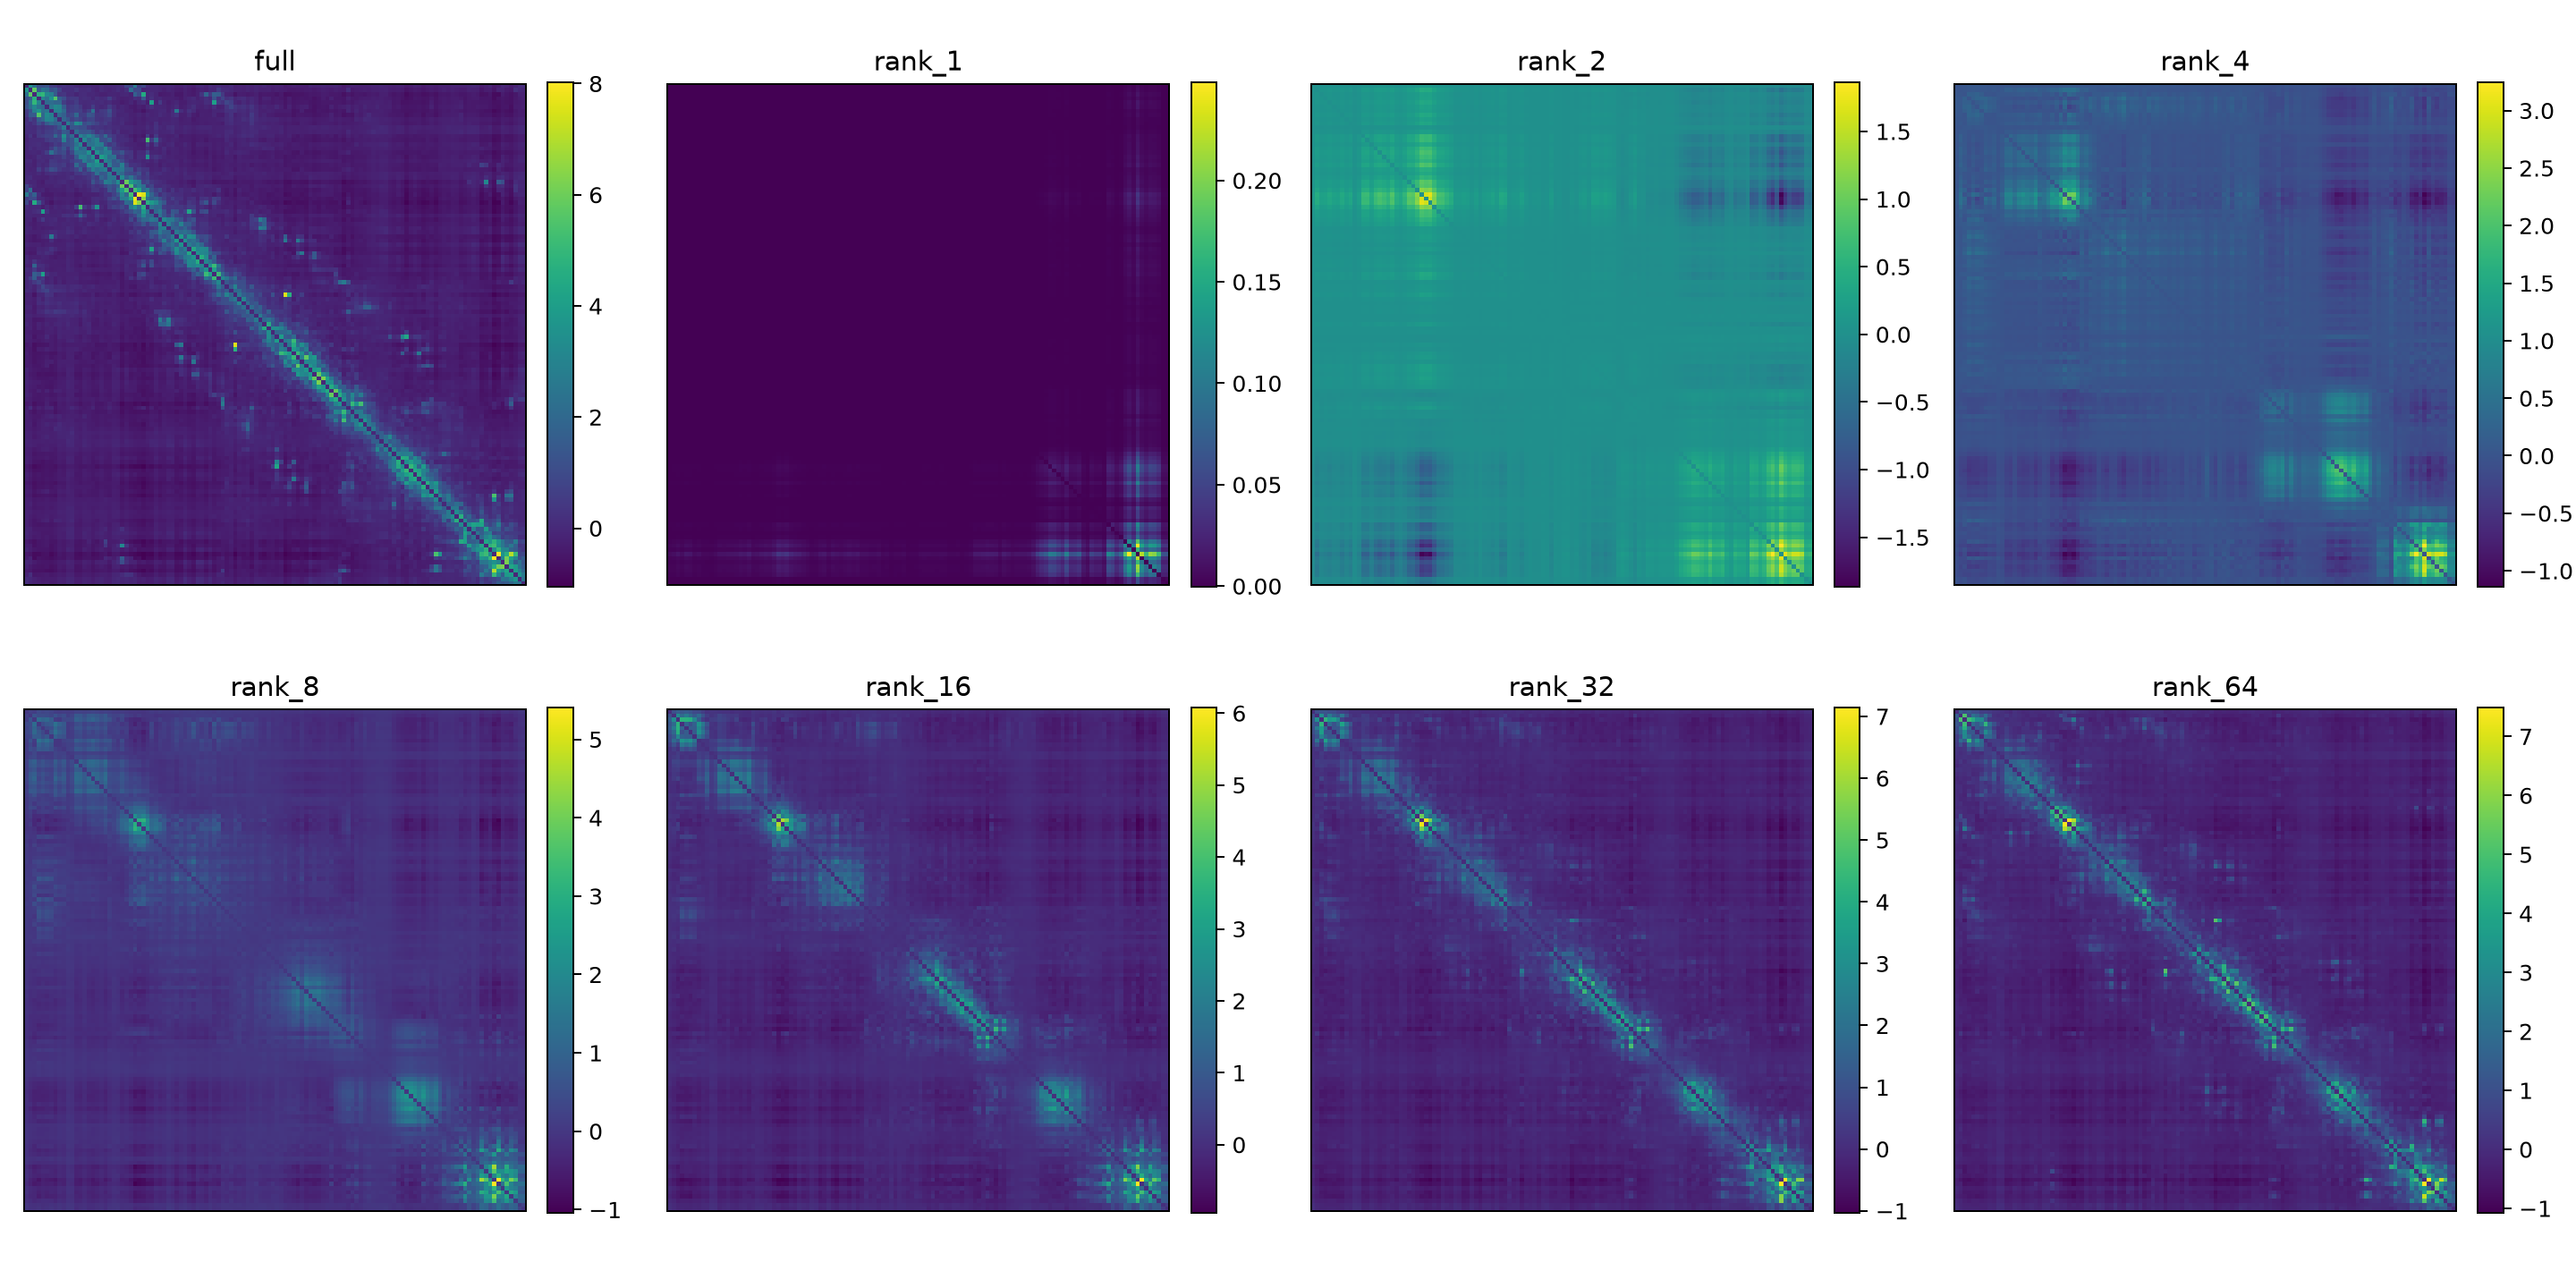
\includegraphics[width=\linewidth]{figures/categorical_compression_maps.png}
\caption{Oracle low-rank reconstruction of the centered symmetric categorical response under
the initial uniform-gauge diagnostic.  Rank one is dominated by a broad background pattern;
structural detail is recovered across subsequent signed modes.}
\label{fig:compression}
\end{figure}

\subsection{Trainable factor head}

Table~\ref{tab:demo} summarizes the single-protein feasibility experiment.  The ungated
rank-16 model uses global factor magnitude and develops row/column bands.  Separating
categorical shape from pair magnitude through $\gamma_{ij}$ substantially improves contact
recovery.  Rank 32 nearly matches the teacher contact precision.

\begin{table}[ht]
\centering
\small
\begin{tabular}{lrrrrr}
\toprule
Model & Rank & Rel. error & Score $\rho$ & Long $P@L$ & Gate $>0.5$ \\
\midrule
Teacher & -- & 0.000 & 1.000 & 0.800 & -- \\
Ungated factors & 16 & 0.765 & 0.599 & 0.400 & -- \\
Gated factors & 16 & 0.494 & 0.808 & 0.750 & 7.35\% \\
Gated factors & 32 & 0.395 & 0.895 & 0.792 & 6.96\% \\
Gated rank 32, no sparse loss & 32 & 0.395 & 0.901 & 0.767 & 7.08\% \\
\bottomrule
\end{tabular}
\caption{3CNBA factor-head results.  Score $\rho$ is Spearman correlation between predicted
and teacher block-Frobenius maps.  Differences of one or two contacts should not be interpreted
as significant on this single family.}
\label{tab:demo}
\end{table}

For the rank-32 gated model, marginal KL is $2.1\times10^{-5}$, entropy Spearman correlation
is 0.99994, and the maximum weighted-gauge residual is $2.1\times10^{-7}$.  The predicted
score-map leading-mode fraction is 0.314, compared with 0.443 for the teacher.  Ninety percent
of predicted pair-score energy is concentrated in 12.2\% of pairs.

\begin{figure}[t]
\centering
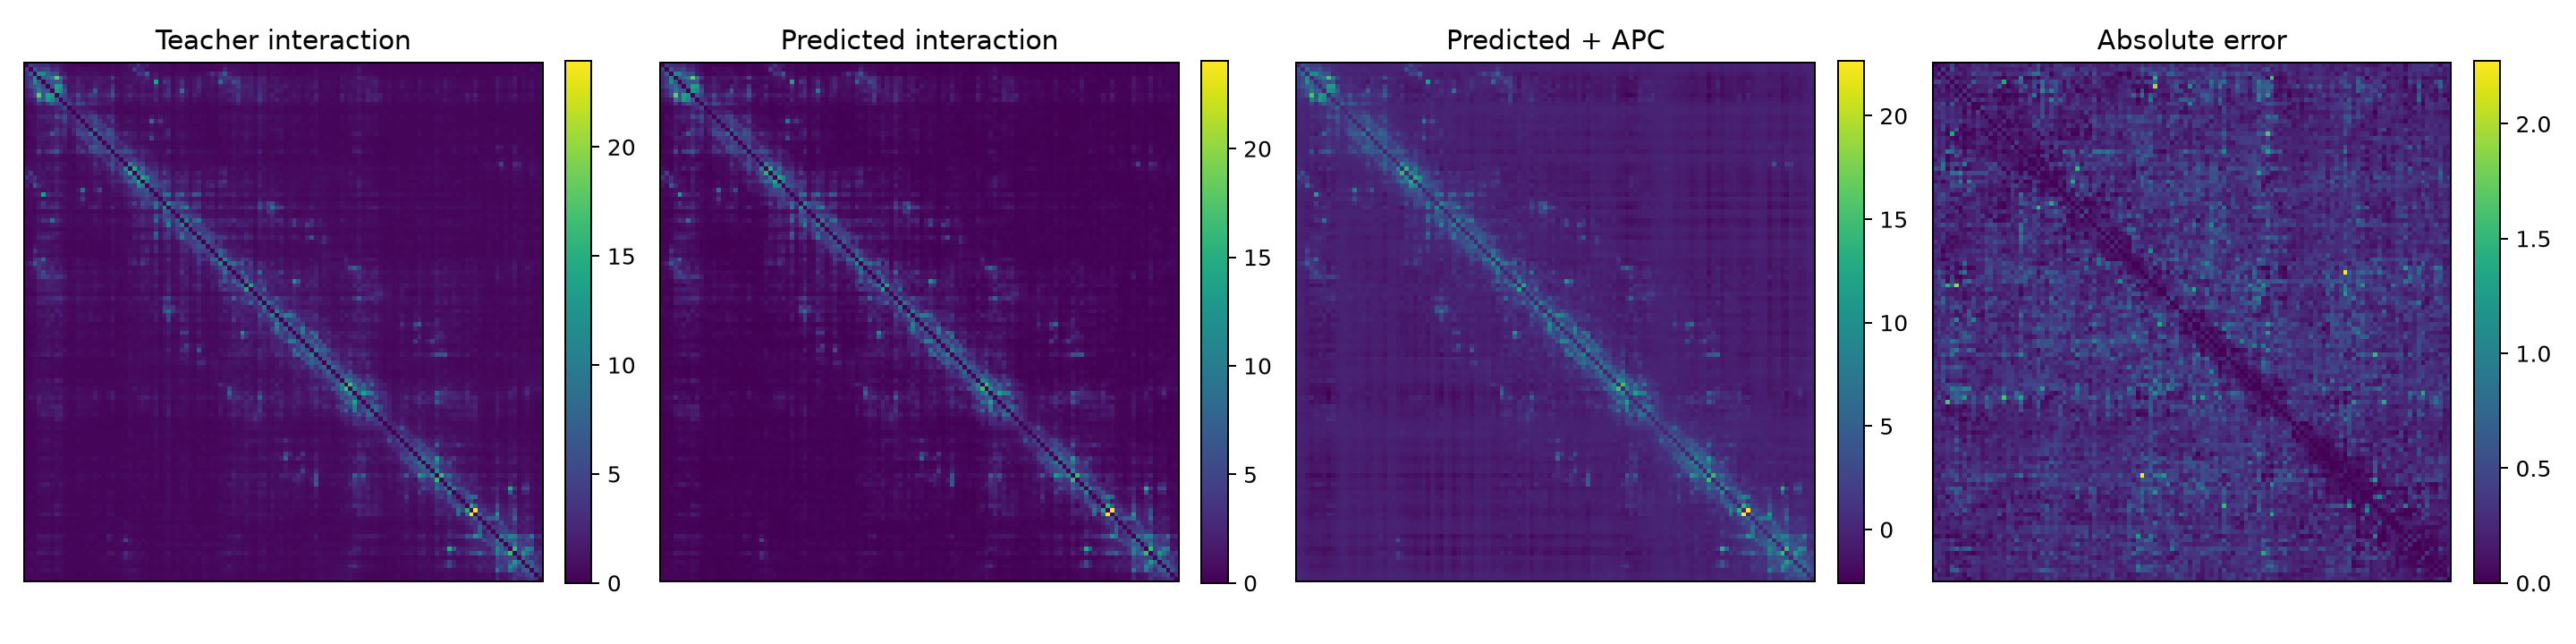
\includegraphics[width=\linewidth]{figures/3cnba_factor_head_maps.png}
\caption{Teacher and rank-32 factor-head interaction maps.  The trainable head receives only
the single query representation at inference; the MSA PSSM and finite-mutation tensor are
training teachers.}
\label{fig:factor-head}
\end{figure}

\subsection{Entropy correlation is not leakage by itself}

The teacher pair-score row strength has Spearman correlation $-0.802$ with MSA entropy.
The learned gate has correlation $-0.802$ as well.  Penalizing this correlation slightly changes
contact rankings but does not provide a principled separation: conserved sites can participate
in more or stronger structural constraints.  We therefore retain Eq.~\ref{eq:orthogonality} as
the hard disentanglement condition and treat scalar entropy correlation only as a diagnostic.

\subsection{Held-out-family benchmark}

We next use 383 protein families with a mean aligned length of 186 and mean effective depth
near 960.  Query-gap columns are removed consistently from sequences, MSAs, and contact
maps.  Families are clustered when query identity is at least 25\% at 80\% bilateral coverage;
no cluster crosses data roles.  The resulting split contains 245 training, 24 calibration,
57 validation, and 57 test families.  A single rank-32 head is trained on frozen ESM-2 8M
states.  MSAs generate sampled teachers only during training and evaluation; inference of the
student head receives one sequence.

The first shared-head experiment uses connected categorical covariance with a sigmoid gate.
It fails in the predicted way: 92.3\% of test gates exceed 0.5 and the score-map leading-mode
fraction is 0.980.  Weighted categorical orthogonality prevents one-body leakage inside each
$20\times20$ block but does not prevent a dense background across position pairs.

Hard-thresholding Eq.~\ref{eq:entropy-null} at three MADs is also suboptimal.  A nonlinear
pair indexer predicts the binary residual with ROC AUC 0.665 but reaches contact $P@L=0.044$.
Training the same model on the continuous robust score raises contact $P@L$ to 0.063.  The
paired improvement over the current typed head is 0.010, with 95\% bootstrap interval
$[0.003,0.017]$.  Bilinear and pair-MLP continuous indexers perform similarly, indicating that
the teacher objective matters more than modest indexer capacity.

\begin{table}[t]
\centering
\small
\begin{tabular}{lrrr}
\toprule
Model/objective & Long $P@L$ & Teacher score $\rho$ & Block rel. error \\
\midrule
Bilinear, binary & 0.058 & -- & -- \\
Pair MLP, binary & 0.044 & -- & -- \\
Bilinear, continuous & 0.062 & 0.244 & -- \\
Pair MLP, continuous & 0.063 & 0.324 & -- \\
Global-mode typed top-$k$ & 0.035 & 0.299 & 1.039 \\
Pair-conditioned typed top-$k$ & 0.045 & 0.324 & 1.088 \\
Pair-conditioned, phylogeny-4 & 0.045 & 0.324 & 1.076 \\
\bottomrule
\end{tabular}
\caption{Mean results on 57 held-out test families.  Long-range contact prevalence is 0.026.
Continuous entropy-normalized routing generalizes, whereas direct reconstruction of empirical
categorical covariance remains unsuccessful even with pair-conditioned modes.}
\label{tab:family-results}
\end{table}

For the MSA teacher itself, entropy normalization raises long-range $P@L$ from 0.094 to
0.102.  Removing four sequence-level PCA modes raises sampled contact average precision from
0.084 to 0.097; the paired 95\% interval for the improvement is $[0.002,0.023]$.  Removing
sixteen modes lowers ROC AUC by 0.030, showing that low-rank subtraction must remain shallow.
The cleaner categorical teacher nevertheless does not make full block prediction learnable from
frozen single-sequence states.

\begin{figure}[t]
\centering
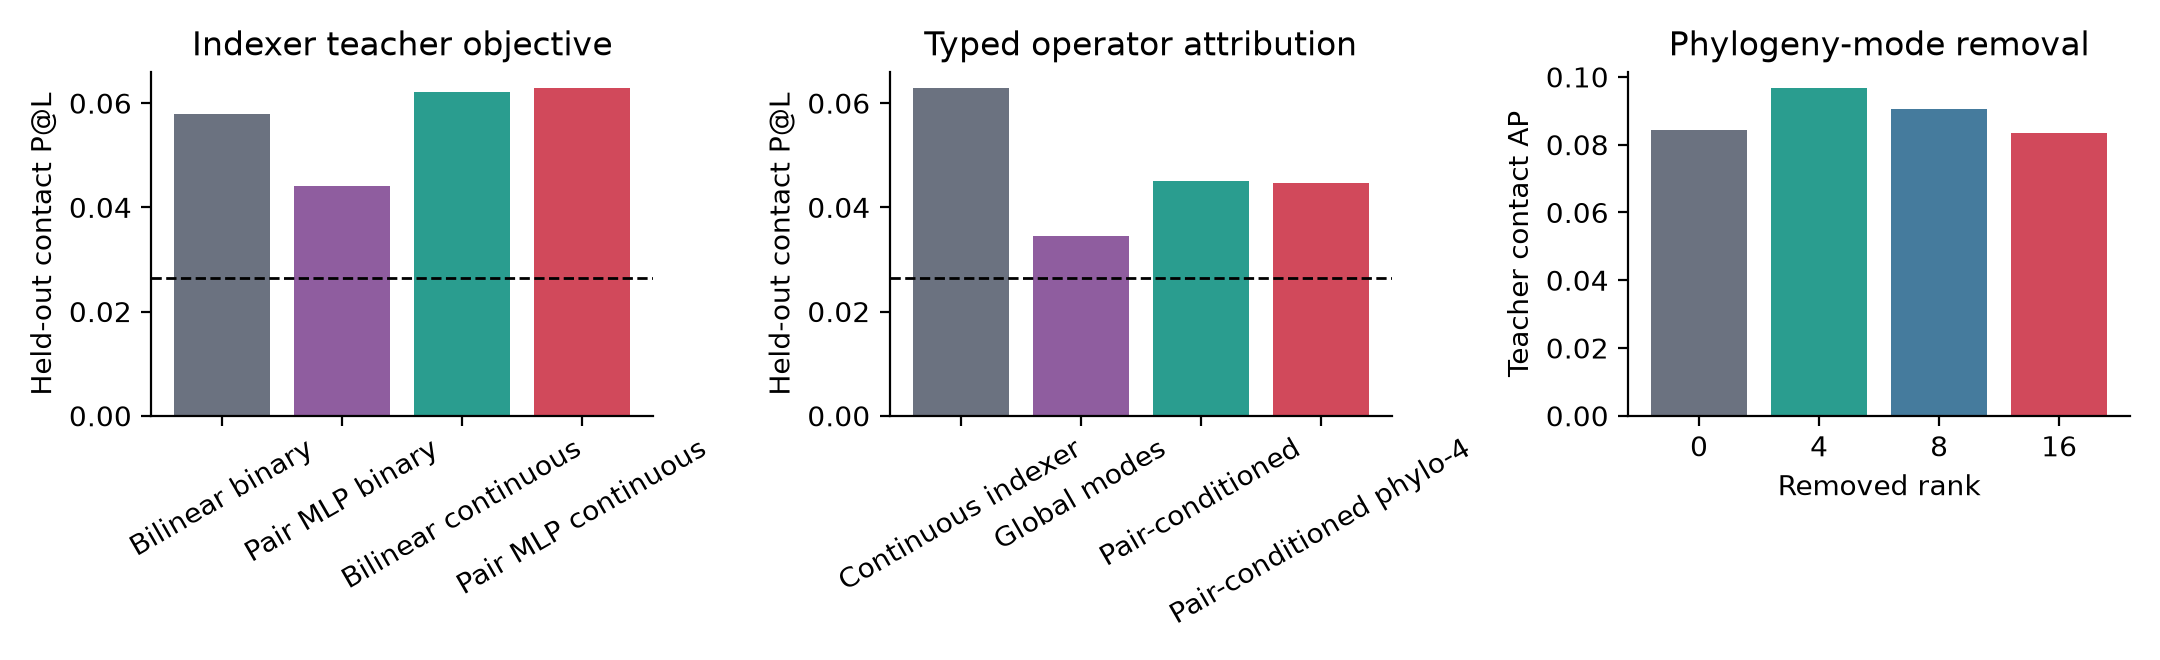
\includegraphics[width=\linewidth]{figures/architecture_revision.png}
\caption{Architecture attribution on held-out families.  Continuous relation distillation is
superior to hard binary routing.  Pair-conditioned modes improve over global modes but remain
below the indexer ceiling.  Removing four phylogeny modes improves the MSA teacher, whereas
aggressive removal destroys signal.}
\label{fig:architecture-revision}
\end{figure}

These results change the execution contract of the proposed layer.  The verified component is
continuous sparse routing.  The typed operator should be trained through Eq.~\ref{eq:additive-logits}
on MLM, mutation, or downstream task loss; MSA block reconstruction is retained only as an
auxiliary diagnostic.  A runnable implementation of this layer now satisfies the weighted-gauge
invariant and produces exactly zero interaction message when all selected neighbors are masked.

\subsection{End-to-end masked-language-model demo}

We train one-layer width-64 models on individual sequences sampled from training-family MSAs;
each execution receives only one sequence.  Validation uses fixed masks on 57 unseen-family
query sequences.  The local model has 28.0k parameters, the sparse model 46.9k, and a standard
Transformer 73.3k.  The replicated comparison uses 1,600 masked-token updates.  For the sparse model, the first
1,000 updates initialize the local background.  A first hard-top-$k$ experiment adds 1,000
index-only distillation steps and 500 sparse adaptation updates; its ranking loss remains near
random.  We therefore test a second schedule with 300 dense soft-routing updates followed by
300 hard-top-$k$ adaptation updates.  This path uses no MSA teacher.  Interaction amplitude
starts near zero.

\begin{table}[t]
\centering
\small
\begin{tabular}{lrrr}
\toprule
Model & Parameters & Seed 1 CE & Seed 2 CE \\
\midrule
Local background & 27,988 & 2.93286 & 2.89075 \\
Sparse disentangled & 46,862 & 2.92565 & 2.88837 \\
Transformer & 73,300 & 2.91439 & 2.86723 \\
\bottomrule
\end{tabular}
\caption{Replicated end-to-end demo on held-out families after 1,600 masked-token updates.
The sparse and local losses are not statistically distinguishable in either seed; the
Transformer is significantly better.}
\label{tab:end-to-end-demo}
\end{table}

For the two seeds, paired sparse-minus-local intervals are $[-0.0151,0.0012]$ and
$[-0.0113,0.0066]$.  Typed interaction contributions, measured as total minus background
cross-entropy, are $-0.00490$ and $+0.00010$: the direction is not reproducible.  Transformer
minus local is significant in both seeds.  Dense soft routing has entropy near 4.85 nats,
showing a distributed warm-up.  Immediate top-$k$ conversion increases loss by 0.00481 and
0.00042; sparse adaptation recovers this loss.  However, index contact $P@L$ remains near
prevalence, so the task-learned routing is not a structural contact predictor.

We then freeze the local background and train only the residual branch with
Eq.~\ref{eq:task-gradient}.  The pair field improves cross-entropy by 0.00416 and 0.00628 in
the two seeds.  Averaging the two seeds within each family gives improvement 0.00522 with
95\% interval $[0.00164,0.00888]$.  The learned field has positive but small mean cosine
alignment, 0.022, with the projected task gradient.

This result does not establish pairwise value.  A site-only residual MLP obeying
Eq.~\ref{eq:site-residual}, with no routing or remote token access, improves loss by 0.00376
and 0.00662.  The paired typed-minus-site difference averaged over seeds is $-0.00003$ with
95\% interval $[-0.00265,0.00256]$.  The two models are statistically indistinguishable.

\begin{figure}[t]
\centering
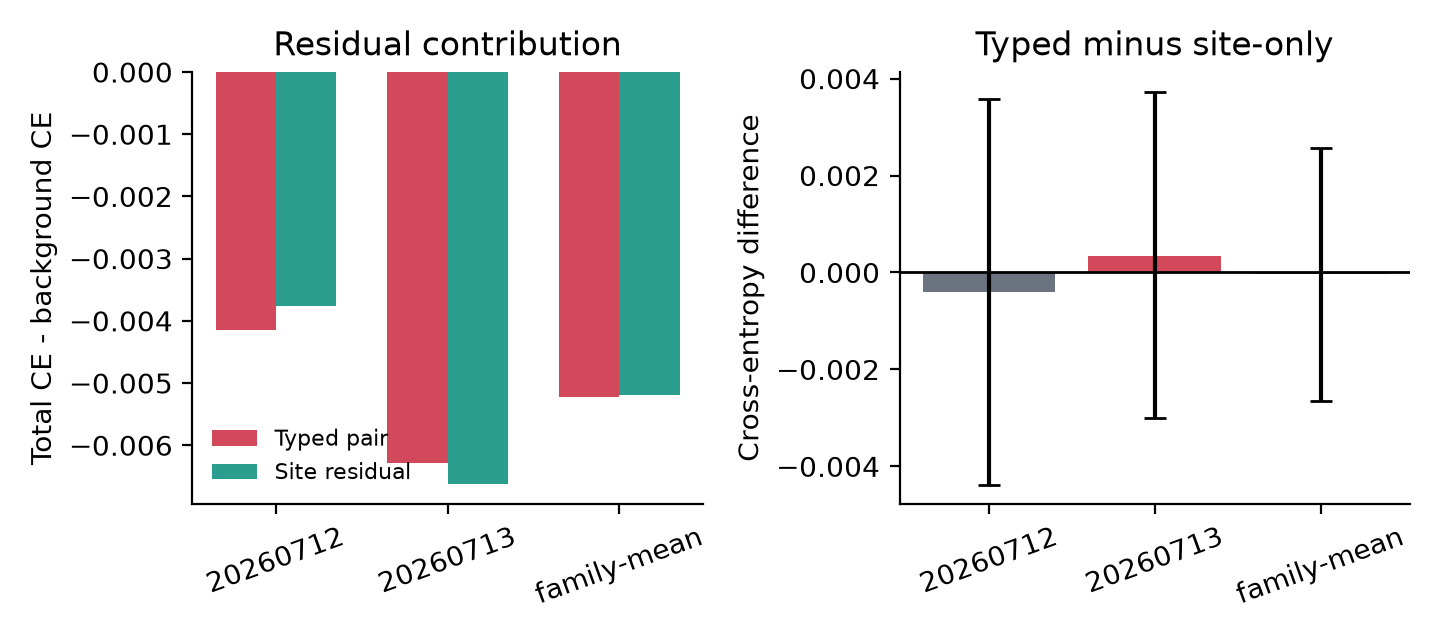
\includegraphics[width=0.82\linewidth]{figures/typed_vs_site_residual.png}
\caption{Task-gradient residual attribution.  Both typed pair and site-only residual branches
improve a frozen background, but their difference is indistinguishable from zero.  The verified
gain comes from marginal-orthogonal residual learning, not from pair structure.}
\label{fig:typed-vs-site}
\end{figure}

\subsection{Identifiable double-mutation epistasis shape}

We freeze the width-64 Transformer demo as a nonlinear teacher.  For each query sequence,
we hold a set of masked probe positions fixed, mutate two unmasked context positions, and
compute Eq.~\ref{eq:epistasis} from the teacher probe loss.  Training uses only query sequences;
no MSA enters this target.  We sample eight pairs and five amino-acid states per family, using
64 training, 24 calibration, and 24 held-out validation families.  Pair regressors receive frozen
single-sequence ESM-2 8M states.  The three matched objectives are a row-plus-column site-only
field, an unconstrained rank-8 pair field, and the same pair field after two-sided weighted
projection.

The physical target RMS varies by more than two orders of magnitude across families.  A single
global amplitude fit is unstable and does not reproducibly beat the zero predictor.  To isolate
interaction geometry, we therefore divide each family target by its RMS and fit one non-negative
output scale on the independent calibration families.  This normalization is a diagnostic, not
an inference-time solution: a deployable model must predict the amplitude in
Eq.~\ref{eq:amplitude-shape} from the single sequence.

Across two seeds, the site-only model explains $-0.18\%$ and $-0.05\%$ of held-out shape
variance.  The unconstrained pair model explains 9.14\% and 6.26\%, while the projected pair
model explains 6.16\% and 4.17\%.  Averaging seeds within family, the projected-pair MSE
improvement over site-only is 0.0528 with a 95\% family-bootstrap interval
$[0.0168,0.0875]$.  Its maximum weighted-gauge error is about $5\times10^{-8}$, versus
0.29--0.64 for the unconstrained pair model.  The projected-minus-unconstrained improvement
is $-0.0253$ with interval $[-0.0500,0.0017]$: exact identifiability currently costs some fit,
although that cost is not resolved at 95\% confidence.

\begin{figure}[t]
\centering
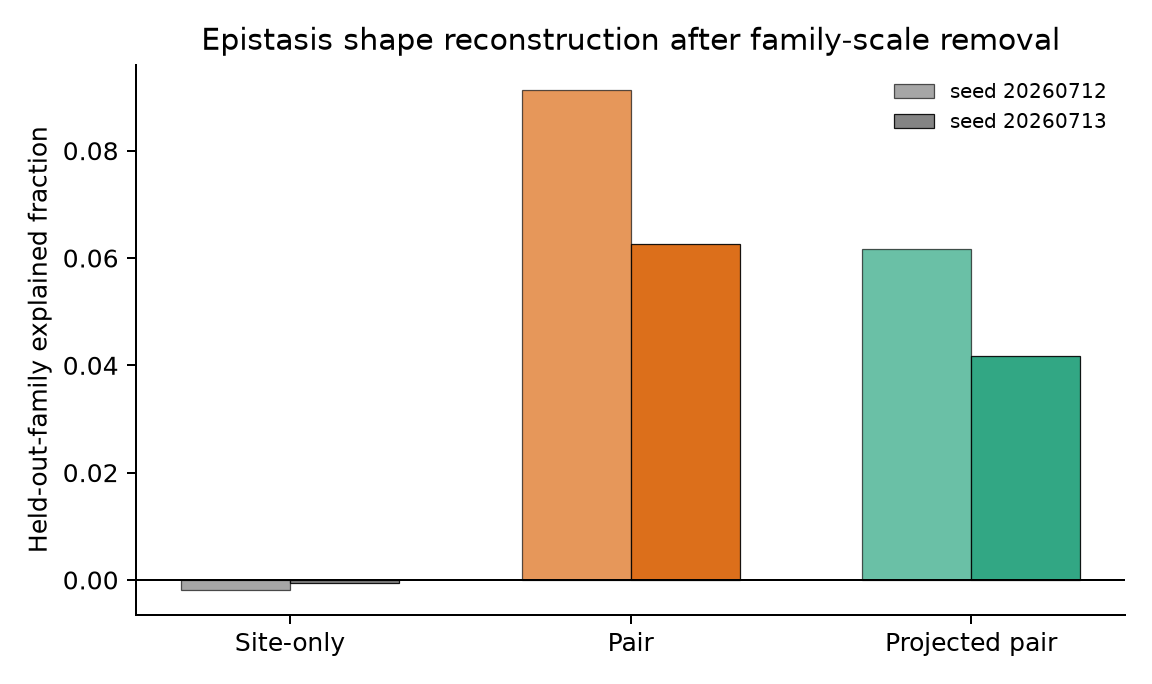
\includegraphics[width=0.88\linewidth]{figures/epistasis_shape_replication.png}
\caption{Held-out-family reconstruction of family-normalized double-mutation epistasis shape.
Only pair models improve over zero; two-sided projection retains a significant gain while
enforcing the weighted gauge to numerical precision.}
\label{fig:epistasis-shape}
\end{figure}

We separately test whether a static strength gate can recover physical interaction magnitude.
For pair strength $s_{ij}=\|\Delta_{ij}\|_{\mathrm{RMS}}$, we fit
\begin{equation}
\log s_{ij}=\mu_{\mathrm{family}}+f_{\mathrm{ent}}(p_i,p_j,|i-j|)+r_{ij},
\label{eq:strength-decomposition}
\end{equation}
where $r_{ij}$ is the proposed sparse routing score.  Small pair MLPs receive frozen ESM states
and are trained either directly on family-standardized log strength or on the residual after
$f_{\mathrm{ent}}$.  Using all 245 training and 57 validation families, the direct-pair top-10\%
average-precision improvement over entropy-only is 0.0122 with 95\% paired interval
$[-0.0233,0.0492]$; Spearman improvement also crosses zero, while MSE is significantly worse
by 0.0889.  The entropy-plus-pair model is likewise negative.  Thus normalized categorical
shape transfers, but physical strength is not recoverable by the tested static frozen-state gate.

We then replace only the gate input with hidden states from the teacher's current masked-task
forward pass.  The dynamic gate reaches held-out Spearman 0.725 and 0.700 and top-10\% average
precision 0.651 and 0.644 in two seeds.  Relative to the static pair gate, family-paired
improvements are 0.698 for Spearman with 95\% interval $[0.655,0.738]$, and 0.445 for average
precision with interval $[0.402,0.491]$.  In contrast, using the same dynamic state for projected
categorical shape gives no reliable advantage over stable ESM values: MSE improvement is
$-0.0083$ with interval $[-0.0599,0.0430]$.

\begin{table}[ht]
\centering
\small
\begin{tabular}{lrrrrrr}
\toprule
Gate input & $\rho_1$ & $\rho_2$ & AP$_1$ & AP$_2$ & MSE$_1$ & MSE$_2$ \\
\midrule
Entropy only & 0.026 & 0.014 & 0.199 & 0.181 & 1.174 & 1.234 \\
Static pair state & 0.034 & -0.005 & 0.199 & 0.205 & 1.253 & 1.332 \\
Dynamic task state & 0.725 & 0.700 & 0.651 & 0.644 & 0.586 & 0.626 \\
\bottomrule
\end{tabular}
\caption{Held-out-family strength routing.  The target is family-standardized log epistasis
RMS.  Dynamic and static gates use the same small pair-MLP budget; only the input state differs.}
\label{tab:dynamic-strength}
\end{table}
\FloatBarrier

\section{Relation to efficient Transformer architectures}

MLA demonstrates that low-rank channel compression can preserve attention quality while
reducing KV cache.  DSA demonstrates that a narrow indexer can distill dense attention and
select a fixed top-$k$ subset.  DeepSeekMoE and Engram demonstrate that common/static
knowledge should not consume the same expensive computation as specialized/dynamic
processing.  NSA adds a crucial systems result: sparsity becomes useful only when its access
pattern is blockwise, natively trained, and matched to hardware.  However, its sequence-block
assumption is a data hypothesis, not a universal property of sparse interactions.  The
implemented dual-stream prototype is
\begin{align}
s_{ij}^{\ell}&=f_{\mathrm{index}}(Q_i^\ell,Q_j^\ell),\qquad
\widehat G_{ij}^{\ell}=f_{\mathrm{value}}(V_i^\ell,V_j^\ell;p_i,p_j),\\
V^{\ell+1}&=V^\ell+F_{\mathrm{background}}^\ell(V^\ell)+\Pi_V I^\ell,\qquad
Q^{\ell+1}=F_{\mathrm{task}}^\ell(Q^\ell,V^\ell)+\Pi_Q I^\ell.
\label{eq:dual-stream}
\end{align}
The task state $Q$ generates routing keys; the slower content state $V$ generates marginals and
typed values.  The index selects top-$k$ pairs, and $I$ evaluates Eq.~\ref{eq:additive-logits}
only on that set.  Only the
typed field is required to obey weighted categorical centering and block-transpose symmetry.  The
local path retains directional context and static motif processing.  DSA-style top-$k$ routing
is prior art; the proposed distinction is that keys and values have different statistical roles:
the key score is entropy-normalized and continuous, while the value is a marginal-orthogonal
signed categorical field.

\subsection{Adaptive-rank ablation}

We tested whether the rank-eight value field could be replaced by a task-conditioned mode gate.
An unregularized gate reaches participation-ratio rank 5.13/5.06 in two seeds. It increases
shape correlation relative to fixed rank eight by 0.00539 with paired 95\% interval
$[0.00129,0.00986]$, while its shape-MSE change and CE-gain change are unresolved. Its
teacher-KL gain is smaller by $6.14\times10^{-5}$ with interval
$[2.72\times10^{-6},1.65\times10^{-4}]$ in favor of fixed rank eight.

The apparent rank reduction is not pair-specific sparsity. Across 1,536 validation pairs per
seed, gate vectors have mean cosine similarity 0.993/0.990 to a seed-specific global template,
and one or two modes dominate the largest gate. Explicit rank penalties reduce effective rank
to approximately three but significantly damage shape reconstruction. A true fixed rank-five
model reduces parameters from 67,022 to 62,927, yet its mean shape-correlation change is
$-0.052$ with substantial seed heterogeneity. Since soft gates still evaluate all eight modes,
they do not reduce runtime. We therefore retain fixed rank eight and do not treat adaptive rank
as a supported architectural contribution.

\subsection{Non-quadratic candidate retrieval}

The symmetric index admits the exact MIPS form
$s_{ij}\propto[r_i,l_i]^\top[l_j,r_j]$.  We therefore tested multi-table random-hyperplane
hashing with Hamming-one probing, followed by exact scoring of retrieved candidates.  The most
faithful configuration evaluates 70.7\% of valid pairs and recovers 97.7\% of dense top-eight
neighbors.  Its message cosine is 0.985, and its CE-gain difference versus dense is
$-7.6\times10^{-5}$ with family-clustered 95\% interval
$[-7.63\times10^{-4},5.23\times10^{-4}]$.  This reduction is too small to offset the hash
projections reliably.  At approximately half of pair evaluations, recall falls to 91.2\%,
message cosine to 0.926, and family-level CE tails become large.

A learned 2,048-parameter shared hash adapter was trained with dense-index distillation,
conditional-response supervision, straight-through binary codes, bit balance, and decorrelation.
It performs worse: 82.4\% neighbor recall at 50.3\% pair evaluation, message cosine 0.860, and
CE-gain difference $-0.00195$ on its first formal seed.  We stop this path and do not insert LSH
into the default layer.

We next trained a contiguous-segment hierarchy and jointly adapted its router, task stream,
index, and value branches while freezing the marginal background.  With beam 16 and 64 exact
candidates, estimated vector work is 62.3\% of dense.  Across two seeds, dense-neighbor recall
is 0.925 with 95\% seed--family--example bootstrap interval $[0.896,0.951]$, and message cosine
is 0.914 with interval $[0.834,0.978]$.  Routed teacher-KL gain is positive in both seeds, with
mean 0.001349 and interval $[0.000433,0.002488]$.  True-residue CE is not stable: routed gains
are 0.01338 and $-0.000649$, producing a mean of 0.00637 with interval
$[-0.00515,0.02334]$.  Thus joint sparse adaptation reconstructs teacher messages, but does not
yet establish a biological-task improvement.

\subsection{Are protein interactions sequence-block sparse?}

The segment hierarchy assumes that important partners occupy contiguous primary-sequence
blocks, as in NSA.  We tested this assumption independently of the learned router.  For 24
held-out families and 96 masked targets, we enumerated every nonlocal context position and all
20 amino-acid substitutions, projected each conditional-response block using
Eq.~\ref{eq:weighted-gauge}, and defined sparse signal as positive interaction energy above the
per-target median.  At a budget of 32 positions, an oracle selecting four arbitrary,
non-overlapping width-eight windows captures 0.616 of total excess energy, versus 0.908 for 32
oracle individual positions.  The block-to-token ratio is 0.674 with family-clustered interval
$[0.637,0.713]$.  Moreover, oracle block mass is only 1.022 times a position-permuted null,
with interval $[1.003,1.043]$.  Width-16 and width-32 blocks perform worse.

\begin{figure}[ht]
\centering
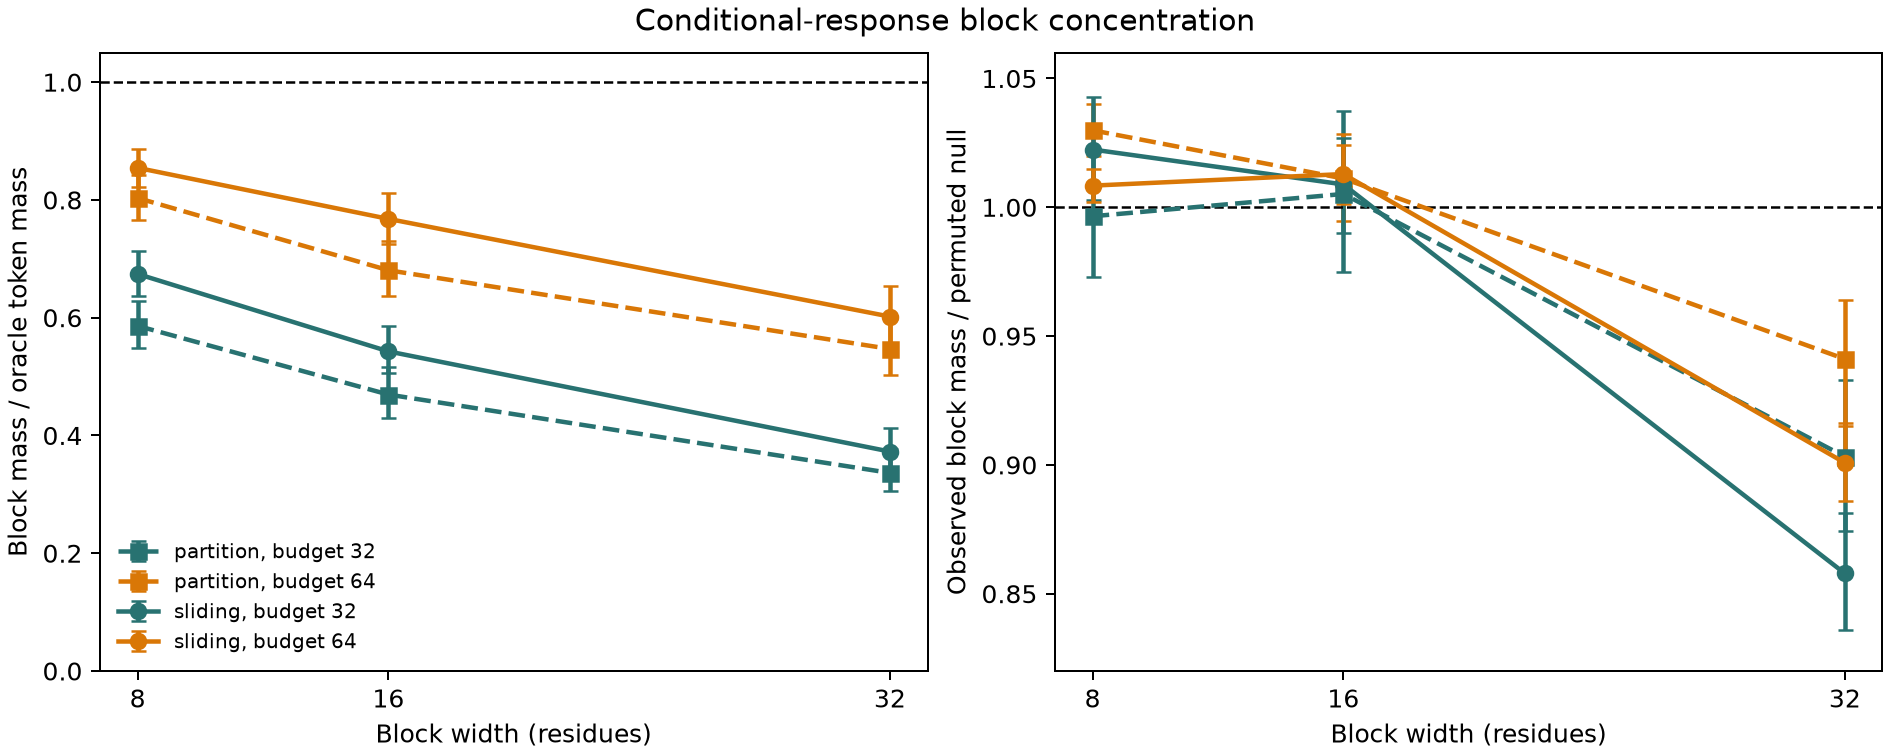
\includegraphics[width=0.98\linewidth]{figures/conditional_block_concentration.png}
\caption{Primary-sequence block concentration of gauge-projected conditional-response energy.
The left panel compares oracle contiguous blocks with an equal-budget oracle that selects
individual positions.  The right panel compares observed block mass with a within-example
position-permuted null.  ``Sliding'' allows arbitrary non-overlapping window starts and is an
upper bound on fixed block partitions.  Error bars are 95\% family-clustered bootstrap
intervals over 24 held-out families and 96 masked targets.}
\label{fig:block-concentration}
\end{figure}
\FloatBarrier

The interaction signal is sparse but has little primary-sequence block concentration.  We
therefore reject contiguous segment leaves as the final candidate representation.

\subsection{Capacity-balanced interaction tiles}

The implemented replacement groups stable keys in learned interaction space.  For stable state
$V_j$, task state $Q_i$, and tile prototype $c_m$, define
\begin{equation}
a_{jm}=\langle W_VV_j,c_m\rangle,\qquad
u_{im}=\langle W_QQ_i,c_m\rangle.
\end{equation}
Sinkhorn normalization converts $a_{jm}$ to an approximately balanced soft assignment $A_{jm}$.
The training-time partner distribution is the tile mixture
\begin{equation}
\widehat P_i(j)=\sum_m \operatorname{softmax}_m(u_i)
\frac{A_{jm}}{\sum_{j'}A_{j'm}},
\label{eq:tile-mixture}
\end{equation}
which is fit to both dense-index and conditional-response distributions.  At execution, a
capacity-constrained hard assignment places at most $\lceil L/M\rceil$ residues in each tile.
Queries rank tiles, collect a fixed candidate budget, evaluate the original exact index only on
those candidates, and decode Eq.~\ref{eq:additive-logits} only for the final top-$k$ neighbors.

The current flat implementation has vector work
\begin{equation}
O(LMd_{\mathrm{tile}}+Lk d_{\mathrm{index}}).
\end{equation}
It validates learned content partitions but is not yet an asymptotic $O(L\log L)$ result when
$M$ grows with length.  A hierarchy over learned tiles is the long-sequence extension.

\begin{table}[ht]
\centering
\small
\begin{tabular}{lrrrr}
\toprule
Router & Candidates & Work ratio & Dense recall & Message cosine \\
\midrule
Segment hierarchy & 32 & 0.344 & 0.732 & 0.786 \\
Segment hierarchy & 64 & 0.623 & 0.910 & 0.895 \\
Content tiles & 32 & 0.285 & 0.967 & 0.969 \\
\bottomrule
\end{tabular}
\caption{Two-seed held-out-validation routing comparison.  Work ratio counts projected tile or
node operations and exact candidate scoring relative to dense exact-index work.  It is an
algorithmic estimate, not a wall-clock speedup.}
\label{tab:tile-routing}
\end{table}
\FloatBarrier

At the same 32-candidate budget, content tiles improve dense-neighbor recall over contiguous
segments by 0.235 with 95\% interval $[0.182,0.286]$, improve message cosine by 0.183 with
interval $[0.040,0.365]$, and reduce estimated work by 0.0593.  Increasing the tile budget from
32 to 64 changes mean message cosine by less than $10^{-4}$ while increasing work from 0.285
to 0.493.

\small
\section{Limitations and next experiments}

The 3CNBA result can be memorized, and direct MSA covariance-block prediction remains near
unit relative error across global, pair-conditioned, and shallow phylogeny-corrected models.
Frozen ESM states may already contain interaction information, and the optional MSA adapter is
not implemented.  The end-to-end sparse demo is tied with its local background and below the
Transformer; soft warm-up solves top-$k$ optimization but not pair-value attribution.

Double-mutation supervision establishes identifiable normalized interaction shape, but the
static strength-gate experiment fails and the system is not end-to-end.  Offline dense
distillation validates the task-conditioned gate, but it still relies on a dense Transformer state.
A linear-cost GRU task stream removes this execution dependency: after 300 dense-teacher and
300 top-$k$ updates, two seeds reach index Spearman 0.595/0.628 and shape correlation
0.164/0.285.  However, interaction-minus-background CE gains are $+0.00218$ and
$-0.00252$; the family-bootstrap mean is $-0.00017$ with interval
$[-0.00471,0.00459]$.

The current value target is semantically misaligned: context--context epistasis affecting a set
of probes is not a direct message to one target site.  The next teacher should instead be
\begin{equation}
R_{ij}(a,b)=\mathcal P_{p_i,p_j}
\left[\ell_i(a\mid x_i=\mathrm{mask},x_j=b)\right],
\label{eq:conditional-response}
\end{equation}
so that $R_{ij}(a,x_j)$ directly supervises the additive message in
Eq.~\ref{eq:additive-logits}.  We tested this teacher in two new runs with a frozen background,
300 dense warm-up steps, and 300 top-$k$ adaptation steps.  The runs reach index Spearman
0.688/0.729 and projected-shape correlation 0.423/0.392.  Relative to the background, teacher
KL improves in both runs; a seed--family--example hierarchical bootstrap gives a mean gain of
$3.84\times10^{-4}$ with 95\% interval $[5.81\times10^{-5},8.50\times10^{-4}]$.
True-residue cross-entropy also improves in both point estimates, but its mean gain is only
0.00151 with interval $[-0.00039,0.00389]$.  Thus the aligned teacher yields reproducible
message distillation, while the task-level gain remains unresolved.  Efficiency claims
additionally require optimized kernels and a matched-compute comparison.

The executable content-tile model replaces that segment router and accepts only a single
sequence.  We evaluated the original categorical value, frozen-value adaptation, and full joint
adaptation at a 32-candidate budget on 57 test families, 12 targets per family, and three model
seeds.  The resulting 2,052 targets are analyzed with a seed--family--example hierarchical
bootstrap.  The original-value router gives dense-neighbor recall 0.970 with interval
$[0.959,0.980]$, message cosine 0.960 with interval $[0.932,0.982]$, and reproducibly positive
teacher-KL gain 0.001230 with interval $[0.000763,0.001692]$.  True-residue CE gain is positive
in all three seeds, with mean 0.002143, but its interval $[-0.001592,0.007546]$ crosses zero.
Frozen-value and full adaptations give CE gains 0.002655 and 0.001963, respectively; neither is
significantly different from the original value.  Full adaptation has negative
routed-minus-dense CE point estimates in all three seeds.  The router therefore generalizes;
additional joint adaptation of the present categorical message objective is not supported.

We also tested whether pairwise addition, rather than the individual value fields, was the
remaining limitation.  A 3,240-parameter permutation-invariant module encodes the eight selected
messages and scores, pools them with the routing weights, and predicts a nonlinear correction:
\begin{equation}
r_i={\cal P}_{p_i}\left[\sum_j w_{ij}m_{ij}
+\psi\!\left(\sum_j w_{ij}\phi(m_{ij},s_{ij})\right)\right].
\label{eq:set-aggregation}
\end{equation}
The final projection preserves the target marginal gauge, and the zero-initialized decoder makes
the initial operator exactly additive.  An unconstrained 1,000-step pilot is unstable: correction
RMS reaches 9.05 times additive RMS and validation performance deteriorates.  We therefore use a
smooth fixed bound of 0.5 times additive RMS and train only the aggregator for 300 steps, with the
backbone, router, index, and categorical value frozen.

Across the same three seeds and 2,052 test targets, the bounded nonlinear correction improves
teacher KL over addition by 0.000523 with interval $[0.000313,0.000823]$, with all seed estimates
positive.  It does not improve the observed residue: nonlinear-minus-additive CE gain is
$-0.001320$ with interval $[-0.004537,0.001108]$, and only one seed is positive.  The correction
uses nearly its full amplitude allowance, with correction-to-additive RMS ratio 0.490 and interval
$[0.482,0.496]$.  The module therefore learns a reproducible teacher-specific direction rather
than failing to optimize.  We retain simple addition and reject the nonlinear aggregator from the
default architecture.

We then measured teacher reliability against the observed residue for each test target.  The
dense Transformer teacher improves CE over the local background by 0.0283 on average, with
interval $[0.0124,0.0441]$, but is better on only 54.2\% of targets, with interval
$[51.2\%,57.2\%]$.  On the 940 teacher-worse targets, the nonlinear-minus-additive CE gain is
$-0.00303$ with interval $[-0.00611,-0.00071]$, even though teacher KL improves.  On the 1,112
teacher-better targets, the CE difference is 0.00050 with interval
$[-0.00355,0.00356]$.  The paired family-stratum contrast is 0.00353 with interval
$[0.00101,0.00578]$.  Closer teacher matching is therefore harmful specifically where the
teacher is wrong.

As a training intervention, we applied KL distillation only when the teacher had lower
training-target CE than the background, while retaining true CE and the gauge constraint for
every example.  On independent test, this reliability gate changes nonlinear CE gain relative
to ungated training by only $-0.000067$, with interval $[-0.000824,0.000780]$.  It reduces
teacher-KL gain by $-0.000400$ with interval $[-0.000593,-0.000270]$ but does not transform that
reduction into task improvement.  Hard teacher filtering is therefore a valid diagnostic but a
failed intervention.  Optional MSA or Transformer supervision should define candidate
interaction directions and must be calibrated independently before setting message amplitude.

We finally tested cross-teacher consensus.  Probability averaging between two independently
initialized Transformer teachers improves masked-residue CE over the first teacher by 0.00838,
with interval $[0.00166,0.01511]$, and gives an absolute background-relative gain of 0.02557 with
interval $[0.00918,0.04178]$.  Agreement itself is not a useful reliability score: cosine
agreement and negative Jensen--Shannon divergence have Spearman correlations only 0.034 and
0.014 with consensus CE gain.

Replacing only the nonlinear aggregator target with the consensus improves its CE point estimate
by 0.00100 relative to single-teacher training, but the paired interval
$[-0.00042,0.00258]$ crosses zero and the model remains below simple addition.  We therefore also
rebuilt the complete conditional-response target: for every context mutation, teacher
probabilities were averaged before taking logarithms and applying the two-sided gauge.  Three
rank-eight models trained from initialization reach shape MSE 0.644, versus 0.806 for the single
teacher, but routing Spearman falls from 0.718 to 0.637.  Consensus interaction CE gain is
0.00143 with interval $[-0.00083,0.00400]$, compared with 0.00131 and interval
$[-0.00047,0.00323]$ for the single teacher.  The paired consensus-minus-single CE difference is
only 0.000126 with interval $[-0.001074,0.001503]$.  A better ensemble predictor and an easier
categorical reconstruction target are therefore insufficient evidence of better interaction
supervision.

We then constructed a non-model evolutionary teacher.  The query row is assigned zero weight;
weighted MSA joint counts are shrunk toward $p_i p_j$, converted to log odds, and projected into
the same two-sided gauge.  Unit-amplitude log odds are miscalibrated, but three independent
validation samplings all select a global message scale of 0.25.  With that scale locked, the
leave-query-out message improves CE on 57 test families and 2,052 targets by 0.05275, with
interval $[0.03207,0.07401]$.  This is the first strong interaction teacher in our experiments.

The failure now moves from supervision to representation.  Rank eight explains 94.1\% of each
MSA block's energy on average, but a left basis shared across all sampled partners of one target
explains only 79.3\%; rank sixteen reaches 96.7\%.  The 300+300-step student obtains validation
index Spearman 0.053 and shape correlation 0.034.  Increasing training to 2,000 dense and 1,000
sparse updates raises shape correlation only to 0.087 and gives CE gain $-0.00130$.  On training
families, index Spearman is 0.863 but shape correlation remains 0.103.  A four-target control can
memorize routing perfectly and reaches shape correlation 0.726, ruling out a broken objective.
The present site-shared categorical factors cannot represent the diversity of evolutionary
fields at this model scale.  The next value operator should create a bounded pair-conditioned
basis residual only after top-$k$ routing, preserving sparse execution and the hard gauge.

\subsection{Routed basis residual: improved memorization, not transfer}

We tested that hypothesis directly.  For each sampled or routed pair, a directional decoder
selects the top two members of an eight-adapter bank and adds the resulting residuals to the
left and right rank-eight categorical factors.  The complete $20\times20$ block, rather than
each adapter separately, is then projected through the two-sided weighted gauge.  Adapter
computation therefore occurs only after pair sampling or top-$k$ routing.

\begin{table}[t]
\centering
\caption{Evolutionary value ablation.  CE gain is background CE minus model CE.  The
memorization column uses four training targets; validation uses 24 unseen families.}
\small
\begin{tabular}{lrrrr}
\toprule
Value model & Params & Mem. $\rho$ & Val. $\rho$ & CE gain \\
\midrule
Shared rank 8 & 67,022 & 0.726 & 0.034 & $-0.000510$ \\
Pair residual rank 8 & 71,959 & 0.776 & 0.056 & $-0.000626$ \\
Balanced residual rank 8 & 71,959 & --- & 0.052 & $-0.000593$ \\
Shared rank 16 & 77,942 & 0.860 & 0.060 & $+0.000791$ \\
\bottomrule
\end{tabular}
\label{tab:pair-basis}
\end{table}

Table~\ref{tab:pair-basis} shows that the residual increases same-rank memorization capacity,
but held-out correlations remain small and shared rank 16 performs similarly.  The rank-16 CE
point estimate is positive in one seed, but its teacher KL is worse than background and thus
does not establish reconstruction of the evolutionary message.  Under the longer
2,000-dense plus 1,000-sparse schedule, shared rank 8 reaches shape correlation 0.087 and MSE
1.949, whereas the pair residual reaches only 0.064 and 1.966.  Its CE gain is nearly neutral
at $-0.000061$, because the interaction RMS shrinks to 0.00250 rather than because the teacher
field is recovered.

The adapter diagnostic explains the failure mode.  Without load control, 89.9\% of directed
pair sides choose the same adapter; the effective number of top adapters is 1.39 of 8 and mean
cosine to the global adapter-weight template is 0.908.  We therefore applied the
DeepSeek-V3 principle that a load-control bias affects top-$k$ selection only, while semantic
mixture weights use the unmodified logits.  This raises the effective adapter count to 6.72 and
reduces template cosine to 0.474, but the model suppresses the residual-to-base RMS ratio from
0.155 to 0.044 and does not improve validation shape.  The simple adapter bank is therefore
rejected: routing diversity cannot compensate for missing transferable pair information in two
independent site states.

The next value hypothesis is a persistent sparse relation state.  Once the validated router
selects edges $E$, define
\begin{align}
r_{ij}^{0}&=f_{\mathrm{init}}(V_i,V_j,Q_i,Q_j,\rho_{ij}),\\
m_i&=\sum_{j:(i,j)\in E}\phi(V_j,r_{ij}),\\
r_{ij}^{l+1}&=r_{ij}^{l}+F_r(r_{ij}^{l},V_i,V_j,m_i,m_j),\\
G_{ij}&=\mathcal P_{p_i,p_j}[f_G(r_{ij})].
\end{align}
Here $\rho_{ij}$ is a relative-position feature.  A node--edge--node update lets each relation
gather context before categorical decoding, costs $O(Lkd_r)$ for bounded degree $k$, and still
accepts a single sequence at inference.  MSA log odds supervise the relation field only during
training.  This operator must beat the factor baselines on held-out shape and teacher KL before
larger-scale training is justified.

\section{Conclusion}

The evidence supports a three-part design: background marginals, a separately calibrated
interaction-strength gate, and a signed marginal-orthogonal interaction shape.  Continuous
relation indexing generalizes, whereas direct MSA covariance reconstruction does not.  Ordinary
MLM validates orthogonal residual learning but not pair structure; an explicitly non-additive
teacher does reveal a small replicated held-out pair signal after amplitude removal.  Sparse
routing is predictable from the current task state but not from a static residue state, while
categorical value shape favors the stable stream.  This supports a dual-stream key/value
separation.  A linear-cost task stream and top-$k$ conversion are trainable, but the present
context--context epistasis teacher does not yield a reproducible message-level CE gain.  Direct
conditional-response supervision repairs the attribution mismatch and reproducibly improves
teacher KL, but its true-residue CE interval still crosses zero.  Matched-compute validation and
optimized sparse kernels remain necessary before the system can be considered a Transformer
replacement.  Soft effective-rank gating is not sufficient: it mostly learns a global mode
reweighting and does not skip computation, while a true fixed rank-five value field is unstable.
Post-hoc and learned LSH candidate routing also fail to provide a reliable low-budget replacement
for the dense index.  A segment hierarchy recovers dense messages more faithfully, but protein
conditional responses do not exhibit the primary-sequence block concentration assumed by that
router.  Capacity-balanced content tiles solve the candidate-retrieval problem at the tested
lengths: 32 candidates retain 97.0\% dense-neighbor recall on an independent split at about
31.8\% estimated vector work.  The three-seed CE point estimate is positive but remains
statistically unresolved, and neither frozen-value nor full joint adaptation improves it
significantly.  The supported architecture therefore keeps a stable marginal-orthogonal value
path and adapts the dynamic router separately.  A bounded gauge-preserving nonlinear set
aggregator reliably matches the conditional-response teacher more closely but moves true-residue
CE in the wrong direction on average, so additional aggregation capacity is not supported either.
Target-level analysis confirms that this harm concentrates where the teacher is worse than the
background, but hard reliability-gated distillation still does not improve independent CE.  The
same conclusion holds for cross-teacher consensus: it improves ordinary masked-residue prediction
and categorical reconstruction error but not interaction CE.  The next scientific bottleneck is
therefore no longer the absence of a useful target: calibrated leave-query-out MSA log odds give
a strong independent CE oracle.  The bottleneck is a value parameterization that can transfer
those pair-specific categorical fields from single sequences.  A sparse pair-conditioned basis
residual improves memorization but not transfer, even after an auxiliary-loss-free load-control
bias prevents adapter collapse.  The next architectural hypothesis is therefore a persistent
sparse relation-state stream, while the next systems bottleneck remains a hierarchical tile
kernel with measured wall-clock speedup.

\scriptsize
\begin{thebibliography}{9}

\bibitem{wang2024disentanglement}
H.~Wang et al.
\newblock Disentanglement of evolutionary constraints in statistical models of proteins.
\newblock \emph{PRX Life}, 2024.

\bibitem{deepseekmoe}
D.~Dai et al.
\newblock DeepSeekMoE: Towards ultimate expert specialization in mixture-of-experts language models.
\newblock arXiv:2401.06066, 2024.

\bibitem{deepseekv2}
DeepSeek-AI et al.
\newblock DeepSeek-V2: A strong, economical, and efficient mixture-of-experts language model.
\newblock arXiv:2405.04434, 2024.

\bibitem{deepseekv3}
DeepSeek-AI.
\newblock DeepSeek-V3 technical report.
\newblock arXiv:2412.19437, 2024.

\bibitem{deepseekv32}
DeepSeek-AI.
\newblock DeepSeek-V3.2-Exp: Boosting long-context efficiency with DeepSeek Sparse Attention.
\newblock Technical report, 2025.

\bibitem{engram}
X.~Cheng et al.
\newblock Conditional memory via scalable lookup: A new axis of sparsity for large language models.
\newblock Technical report, 2026.

\bibitem{nsa}
J.~Yuan et al.
\newblock Native Sparse Attention: Hardware-aligned and natively trainable sparse attention.
\newblock arXiv:2502.11089, 2025.

\end{thebibliography}

\end{document}
